\chapter{Z Document Rhetorical aspect}
\label{ch:zdra}
The \gls{zdra} is similar to the \gls{dra} for mathematics. Here we describe how
the \gls{zdra} was designed an implemented. 

We use the ZMathLang \LaTeX{} package to chunk specifications together and see
the relationships between them. The mathematical instances used are
\textit{theory} and \textit{axiom}, which are used in theorem prover syntax. We
also use \textit{precondition}, \textit{postcondition}, \textit{output},
\textit{stateInvariants}, \textit{stateschema}, \textit{outputschema},
\textit{changeschema} and \textit{totaliseSchema}.

We created the ZDRa for the following:

\begin{itemize}

\item Identifying loops in the reasoning of specifications.
\item Checking the specification is robust by making sure schemas have been
totalised.
\item Identifying the relationships between chunks of specification.
\item Making sure state invariants do not change throughout the specification.
\item Creating a dependency graph to create a formal proof sketch from the ZDRa.
\end{itemize}

As well as having instances, the ZDRa shows relations between them to make sure
there are no loops in reasoning and to give warning in some situations (e.g.
specification is not totalised).

Section \ref{sec:zdra_annotate} describes the labels used to annotate a
specification. Then in section \ref{sec:zdra_implement} we illustrate the
implementations of the \gls{zdra} and how to check for rhetorical correctness.
The rhetorical errors which can be found are explained in sections
\ref{subsubsec:zdra_looperrors} and \ref{subsubsec:zdra_toterrors} and the
products which are created when a specification is rhetorically correct are
described in section \ref{subsec:zdra_prodcuts}.

\section{Annotations}
\label{sec:zdra_annotate}

Using our ZMathLang \LaTeX{} package we can label the specifications with
\gls{zdra} annotations (either before of after the \gls{zcga}). These
annotations chunks parts of the specification together and upon compiling shows
the relationships between each of these chunks.

\begin{table}[H]
\begin{tabular}{| c | c | c | c |}
\hline
\textbf{Instance} & \textbf{Notation} & \textbf{\LaTeX{} Command}  \\
\hline
theory & T & $\backslash$dratheory\{\textit{T}\}\\
& & \{\textit{scaleoftheory}\}\{\textit{instance}\}  \\
\hline
stateschema & SS & $\backslash$draschema\{\textit{SS\#}\}\{\textit{instance}\}
\\
\hline
initschema & IS & $\backslash$draschema\{\textit{IS\#}\}\{\textit{instance}\}
\\
\hline
changeschema & CS & $\backslash$draschema\{\textit{CS\#}\}\{\textit{instance}\}
\\
\hline
outputschema & OS & $\backslash$draschema\{\textit{OS\#}\}\{\textit{instance}\}
\\
\hline
totaliseSchema & TS &
$\backslash$draschema\{\textit{TS\#}\}\{\textit{instance}\}  \\
\hline
axiom & A  & $\backslash$draschema\{\textit{A\#}\}\{\textit{instance}\}  \\
\hline
stateInvariants & SI & $\backslash$draline\{\textit{SI\#}\}\{\textit{instance}\}
\\
\hline
precondition & PRE & $\backslash$draline\{\textit{PRE\#}\}\{\textit{instance}\}
\\
\hline
postcondition & PO  & $\backslash$draline\{\textit{PO\#}\}\{\textit{instance}\}
\\
\hline
output & O  & $\backslash$draline\{\textit{O\#}\}\{\textit{instance}\}  \\
\hline
\end{tabular}
\caption{\label{tab:instances} \gls{zdra} instances with their notations and \LaTeX{} commands.}
\end{table}

\begin{table}[H]
\begin{tabular}{| c | c |}
\hline
\textbf{Relation} &  \textbf{\LaTeX{} Command} \\
\hline
initialOf &  $\backslash$initialof
\{\textit{instance\_1}\}\{\textit{instance\_2}\}  \\
\hline
uses & $\backslash$uses \{\textit{instance\_1}\}\{\textit{instance\_2}\}\\
\hline
requires & $\backslash$requires
\{\textit{instance\_1}\}\{\textit{instance\_2}\}\\
\hline
allows & $\backslash$allows \{\textit{instance\_1}\}\{\textit{instance\_2}\}\\
\hline
totalises & $\backslash$totalises
\{\textit{instance\_1}\}\{\textit{instance\_2}\}\\
\hline
\end{tabular}
\caption{\label{tab:relations} \gls{zdra} Relations with their notations and \LaTeX{} commands.}
\end{table}

Table \ref{tab:instances} shows the type of instance available in a Z
specification, the notation that goes along with it and the \LaTeX{} command the
user annotates that part of the specification with. It is important to name
instances as these names are what are referred to when creating the
relationships between them. Table \ref{tab:relations} shows the relationships
which are available between some of the instances. 

\subsection{Instances}

We have designed the notation to include \verb|\draschema{..}{..}| for chunks of
specification which include schemas and \verb|\draline{..}{..}| which only
include lines within a schema.

\subsubsection{theory}

A \emph{theory} would be a whole specification of one particular system.
Appendix ?? shows an entire specification labelled in \gls{zdra}. You can have
more than one \emph{theory} in a single document. The \emph{theory} would
contain all other instances within it but no instance can have a \emph{theory}
inside of it.

\subsubsection{stateschema}

A \emph{stateschema} just like in Z is a single instance which outlines the
state of the system. Figure \ref{fig:exampleofss} shows an example of a
\emph{stateschema} instance. Note we have the label \verb|\draschema{SS1}{....}|
(shown in red) where we have labelled this \emph{stateschema} \verb|SS1|. There
may be one or more \emph{stateschema}'s in a theory. So users can label their
\emph{stateschema}'s accordingly, e.g.
\verb|SS1, SS2,SS3|.....\footnote{Although it is not needed for the user to annotate the
instances incrementally (the instances just need different numbers) it makes it
easier to identify how many of each instance is within the specification.}

\begin{figure}[H]
\centering
\begin{footnotesize}
\begin{BVerbatim}[commandchars=+\[\]]
[+color[red]\draschema{SS1}{]\begin{schema}{BirthdayBook}known: \power NAME \\
birthday: NAME \pfun DATE \where[+color[blue]\draline{SI1}{]known=\dom
birthday[+color[blue]}]\end{schema}[+color[red]}]
\end{BVerbatim}
\end{footnotesize}
\caption{\label{fig:exampleofss} A stateschema and stateinvariants labelled in \gls{zdra}.}
\end{figure}

\subsubsection{initialschema}

An \emph{initialschema} instance is optional within a \emph{theory}, there can
be more than one depending on how many \emph{stateschema}'s there are. Figure
\ref{fig:exampleofis} shows an example of an \emph{initialschema}. We use the
labelling \verb|\draschema{IS1}{...}| (shown in red) to denote the
\emph{initialschema}. We have named the \emph{initialschema} \verb|IS1| to show
it is the first initial schema in the \emph{theory}. If there was another
\emph{initialschema} we would name it \verb|IS2| and so on.

\begin{figure}[H]
\centering
\begin{footnotesize}
\begin{BVerbatim}
    [commandchars=+\[\]] [+color[red]\draschema{IS1}{]
\begin{schema}{InitBirthdayBook} 
BirthdayBook' 
\where 
[+color[blue]\draline{PO2}{]known' = \{ \}[+color[blue]}]
\end{schema}
[+color[red]}]
\end{BVerbatim}
\caption{\label{fig:exampleofis} An initialschema labelled in \gls{zdra}.}
\end{footnotesize}
\end{figure}

\subsubsection{changeschema}

A \emph{changeschema} instance is a schema/function which changes the current
state of the specification (these schemas are usually denoted by having a
\verb|\Delta| operator). There can be none or many \emph{changeschema} instances
within a theory.

\begin{center}
\begin{figure}[H]
\centering
\begin{footnotesize}
\begin{BVerbatim}[commandchars=+\[\]] [+color[red]\draschema{CS1}{]
\begin{schema}{AddBirthday}
\Delta BirthdayBook \\
name?: NAME \\
date?: DATE
\where
[+color[blue]\draline{PRE1}{]name? \notin known[+color[blue]}]
[+color[green]\draline{PO3}{]birthday' = birthday \cup \{name? \mapsto
date?\}[+color[green]}]
\end{schema}
[+color[red]}]
\end{BVerbatim}
\end{footnotesize}
\caption{\label{fig:exampleofcs} A changeschema labelled in \gls{zdra}.}
\end{figure}
\end{center}

Figure \ref{fig:exampleofcs} shows an example of a \emph{changeschema} annotated
in \gls{zdra}. The schema is labelled with: \verb|\draschema{CS1}{...}| (shown
in red). We name this instance \verb|CS1| as it is the first \emph{changeschema}
instance seen in the specification, the next \emph{changeschema} should be named
\verb|CS2| then \verb|CS3| etc.

\subsubsection{outputschema}

An \emph{outputschema} instance is a schema or a function which does not change
the current state but only outputs information from the current state (these
schemas are usually denoted by having a \verb|\Xi| operator). Figure
\ref{fig:exampleofos} shows an example of an \emph{outputschema} instance in
\gls{zdra}. Note the line \verb|\draschema{OS4}{....| (shown in red) which names
the chunk \verb|OS4| that is the forth \emph{outputschema} in the specification.

\begin{figure}[H]
\centering
\begin{footnotesize}
\begin{BVerbatim}[commandchars=+\[\]] [+color[red]\draschema{OS4}{]
\begin{schema}{AlreadyKnown}
\Xi BirthdayBook \\
name?: NAME \\
result!: REPORT
\where
[+color[blue]\draline{PRE3}{]name? \in known[+color[blue]}] \\
[+color[green]\draline{O4}{]result! = already\_known[+color[green]}]
\end{schema}
[+color[red]}]
\end{BVerbatim}
\end{footnotesize}
\caption{\label{fig:exampleofos} A outputschema labelled in \gls{zdra}.}
\end{figure}

\subsubsection{totaliseSchema}

A \emph{totalise} instance are parts of the specification which totalise
preconditions and schemas within the specification. These are labelled as
\verb|TS#| where \verb|#| is some number. \emph{Totoalise} instances can written
in two ways. Either using the double equals operator:

\begin{verbatim}
\begin{zed}
A == B \land C
\end{zed}
\end{verbatim}

or by using the \verb|defs operator|:

\begin{verbatim}
\begin{zed}
A \defs B \land C
\end{zed}
\end{verbatim}

When labelling \emph{totalise} instances the user can do this in two ways. The
first labelling is as a \verb|draschema| where the labelling comes before the
\verb|\begin{zed}| or as a \verb|draline| where the labelling wraps around the
line of the instance only. The second way is useful if there are more than one
\emph{totalise} instance between the \verb|\begin{zed}| and \verb|\end{zed}|. 

\begin{figure}[H]
\centering
\begin{footnotesize}
\begin{BVerbatim}[commandchars=+\[\]] [+color[red]\draschema{TS3}{]
\begin{zed}
VM3 \defs VM1 \lor VM2 \end{zed}[+color[red]}]
\end{BVerbatim}
\end{footnotesize}
\caption{\label{fig:exampleofts1} A totalise schema instance labelled in \gls{zdra}.}
\end{figure}

An example of the \verb|draschema| labelling is shown in figure
\ref{fig:exampleofts1} where we have the label \verb|\draschema{TS3}{..| (shown
in red).

\begin{figure}[H]
\centering
\begin{footnotesize}
\begin{BVerbatim}[commandchars=+\[\]]
\begin{zed} 
[+color[red]\draline{TS1}{]RAddBirthday == (AddBirthday \land Success)\\  \lor
AlreadyKnown[+color[red]}] \\
[+color[red]\draline{TS2}{]RFindBirthday == (FindBirthday \land Success) \lor
NotKnown[+color[red]}] \\
[+color[red]\draline{TS3}{]RRemind == Remind \land Success[+color[red]}]
\end{zed}
\end{BVerbatim}
\end{footnotesize}
\caption{\label{fig:exampleofts2} A totalise line instance labelled in \gls{zdra}.}
\end{figure}

An example of the \verb|draline| instance is shown in figure
\ref{fig:exampleofts2}. In this example we have three \emph{totalise instances}
using the label \verb|\draline{TS1}{...|, \verb|\draline{TS2}{...| and
\verb|\draline{TS3}{...| respectfully (shown in red).

\emph{Totalise} instances become the properties to prove when converted to the
half-baked proof (see section \ref{sec:gpsa2is} for details).


\subsubsection{axiom}

\emph{Axiom} instances are knowns as axiomatic definitions in Z. There can be
more than one \emph{axiom} in a \emph{theory} or there can be none. An example
of an \emph{axiom} instance labelled in \gls{zdra} is shown in figure
\ref{fig:exampleofa}. Note the \gls{zdra} labelling consists if the line
\verb|\draschema{A1}{...| where the instance is named \verb|A1|.

\begin{figure}[H]
\centering
\begin{footnotesize}
\begin{BVerbatim}[commandchars=+\[\]] [+color[red]\draschema{A1}{]
\begin{axdef}
maxPlayers: \nat
\where
maxPlayers = 20 \end{axdef}[+color[red]}]
\end{BVerbatim}
\end{footnotesize}
\caption{\label{fig:exampleofa} A axiom instance labelled in \gls{zdra}.}
\end{figure}

\subsubsection{stateInvariants}
The \emph{stateInvariants} instance are the conditions which must be obeyed
throughout the specifications. These are the lines founds inside the
\emph{stateschema} instance. Figure \ref{fig:exampleofss} shows a single
\emph{stateinvariant} instance labelled as \verb|\draline{SI1}{..| (shown in
blue). There can be 0 or more \emph{stateinvariance} instances within a
\emph{theory}.

\subsubsection{precondition}

Similar to the \emph{totalise} instance, the \emph{precondition} instance can be
labelled as a \verb|draschema| or a \verb|draline|. An example of a
\emph{precondition} which is a line can be found in figures
\ref{fig:exampleofcs} and \ref{fig:exampleofos}. In figure \ref{fig:exampleofcs}
the \gls{dra} labelling for a \emph{precondition} schema is the line
\verb|\draline{PRE1}{..}| (shown in blue). The \emph{precondition} instance is
named \verb|PRE1| and \verb|name? \notin known| is the instance. In figure
\ref{fig:exampleofos} the \gls{zdra} labelling is 
\verb|\draline{PRE3}{..}|(shown in blue) where \verb|PRE3| is the name of the
instance and 
\verb|name?\in known| is the instance.

Another way a \emph{precondition} instance can exists is when an entire schema
only consist of \emph{precondition} instances and nothing else (no post
operations).

\begin{figure}[H]
\centering
\begin{footnotesize}
\begin{BVerbatim}[commandchars=+\[\]] [+color[red]\draschema{PRE1}{]
\begin{schema}{exact\_cash}
cash\_tendered?: \nat
\where
cash\_tendered? = price \end{schema}[+color[red]}]
\end{BVerbatim}
\end{footnotesize}
\caption{\label{fig:exampleofpre} A precondition schema instance labelled in \gls{zdra}.}
\end{figure}

A \emph{precondition} instance which is an entire schema is shown in figure
\ref{fig:exampleofpre}. The \gls{zdra} labelling consists of the line
\verb|\draschema{PRE1}{..| where the name of the instance is \verb|PRE1|.


\subsubsection{postcondition}

The \emph{postcondition} instance can be labelled as a \gls{zdra} line. An
example of this is demonstrated in figure \ref{fig:exampleofcs} (shown in
green), where the name of the instance is \verb|PO3| and the instance itself is
\verb|birthday' = birthday \cup \{name? \mapsto date?\}|.

\subsubsection{output}

An \emph{output} instance can also be labelled as a \gls{zdra} line. An example
of this is shown in green in figure \ref{fig:exampleofos}. The instance in this
case is named
 \verb|O4| and the instance itself is \verb|result! =already\_known|.

\subsection{Relations}
\label{subsec:zdrarelations}

After labelling the instances within a relation the user may then add relations
between parts of the specification. The relationships available are
\emph{initialOf}, \emph{uses}, \emph{requires} and \emph{allows}.

\begin{table}[H]
\begin{tabular}{|lll||lll|}
\hline
\textbf{requires} & & &  & \textbf{uses} & \\
\hline
outputSchema & $\longrightarrow$ & precondition  & outputSchema &
$\longrightarrow$ & stateSchema\\
outputSchema & $\longrightarrow$ & output & changeSchema & $\longrightarrow$ &
stateSchema \\
changeSchema & $\longrightarrow$ & precondition  & stateSchema &
$\longrightarrow$ & stateSchema \\
changeSchema & $\longrightarrow$ & postcondition  & stateSchema &
$\longrightarrow$ & axiom \\
\cline{1-3}
\textbf{totalises} & &  & outputSchema & $\longrightarrow$ & axiom \\
\cline{1-3}
totalise & $\longrightarrow$ & changeSchema  & changeSchema & $\longrightarrow$
& axiom \\
\cline{4-6}
totalise & $\longrightarrow$ & outputSchema & \textbf{allows}  & & \\
\cline{4-6}
totalise & $\longrightarrow$ & totalise  & precondition  & $\longrightarrow$  &
postcondition \\
\cline{4-6}
& &  & \textbf{initialOf} &  &  \\ 
\cline{4-6}
& &  & initialSchema & $\longrightarrow$ & stateSchema \\ 
\hline
\end{tabular}
\caption{\label{tab:relationsallowed} The legal relations between instances. Where $\longrightarrow$ represents the relation.}
\end{table}

Table \ref{tab:relationsallowed} shows the legal relations between each of the
instances for example an \emph{initialSchema} can be an \emph{initialOf} a
\emph{stateSchema} but it wont allow say a \emph{changeSchema} to be
\emph{initialOf} an \emph{initialSchema} etc.

\subsubsection{initialOf}

An \emph{initialschema} instance can be an \emph{initialOf} a \emph{stateschema}
instance. An example of this would be \verb|\initialOf{IS1}{SS1}| where
\verb|IS1| is \emph{initialOf} \verb|SS1|.

\subsubsection{uses}
The \emph{uses} relation can be between \emph{changeSchema}'s,
\emph{outputSchema}'s, \emph{stateSchema}'s and \emph{totalise} instances. For
example, one can say that an \emph{outputSchema} \emph{uses} a
\emph{stateSchema}. To illustrate this the user can add the label
\verb|\uses{OS2}{SS1}|, meaning \emph{outputSchema} OS2, uses \emph{stateSchema}
SS1.

\subsubsection{requires}
The \emph{requires} relation is used between an \emph{outputSchema} or a
\emph{changeSchema} and a \emph{precondition}, \emph{output} or
\emph{postcondition}. If we take the example shown in figure
\ref{fig:exampleofis} we can say that the \emph{initialSchema} \verb|IS1|
\emph{requires} the postcondition \verb|PO2|. Therefore in \gls{zdra} notation
we would write in our \LaTeX{} specification \verb|\requires{IS1}{PO2}|.

\subsubsection{allows}
The \emph{allows} relation is used between \emph{precondition}'s and
\emph{postconditions} or \emph{preconditions} and \emph{outputs}. This relation
describes if an instance allows another instance to occur. That is an instance
can not exist unless pre-conditional requirements are met. An example of where
an \emph{allows} relationship would be useful is in figure
\ref{fig:exampleofos}, where we have a \emph{precondition} \verb|PRE3| (in blue)
and an \emph{output} \verb|O4| (in green). In this case the user would write in
their \gls{zdra} \LaTeX{} file: \verb|\allows{PRE3}{O4}|.


\section{Implementation}
\label{sec:zdra_implement}

The \gls{zdra} program automatically checks for rhetorical correctness of the
specification. To do this it reads the \gls{zdra} annotations created by the
user then if all is correct then the program automatically generates a
\emph{dependency graph} and a \emph{goto graph}. The input for the \gls{zdra}
program is the specification written in \LaTeX{} with the \gls{zdra}
annotations.

\subsection{Checking if a specification is correctly totalised}

The \gls{zdra} program uses regular expressions to read the annotations inputted
by the user to determine whether a specification has been totalised. For example
if we only have a single \emph{precondition} instance (PRE1), in a specification
and a single \emph{totalise} instance (TS1), in a specification and the user has
added the \emph{relation} \verb|totalises{TS1}{PRE1}|, then the specification
will be correctly totalised and there will be a message saying
"\texttt{Specification correctly totalised}". If there exists any preconditions
which the user hasn't annotated with a totalising relation then the \gls{zdra}
program will display a message saying "\texttt{Specification not correctly
totalised}". This message is a warning not an error therefore even if the
specification still has untotalised preconditions the user can still go on with
the next steps of computerisation.

\subsubsection{Errors}
\label{subsubsec:zdra_toterrors}

Table \ref{tab:totalisecorrect} shows examples of 3 specifications (named 1, 2
and 3). Specification 1 shows three \emph{preconditions} being annotated by the
user (PRE1, PRE2 and PRE3), all these preconditions have been annotated with the
relationship \emph{totalises}. Therefore if all preconditions in a schema have a
totalising condition then the specification is correctly totalised.
Specification 2 in the table shows 4 existing preconditions. All but one (PRE2)
precondition have a totalising relationship with a totalise schema. In this
case, PRE2 is an outstanding preconditions to be totalised and therefore the
message `\texttt{Specification incorectly totalised} appears. Specification 3 in
table \ref{tab:totalisecorrect} shows 5 schema preconditions. When checking
totalising correctness it does not matter whether the preconditions are in
\verb|draline| form or \verb|draschema| form. In the third example we see that
PRE3 and PRE4 have not been totalised and again a message appears saying the
specification has not been correctly totalised.

\begin{table}[H]
\begin{tabular}{|c|c|c|c|}
\hline
& \textbf{Preconditions in} & \textbf{Totalises in} & \textbf{Outcome of} \\
& \textbf{specification} & \textbf{specification} & \textbf{\gls{zdra} program}
\\
\hline
\hline
& \verb|\draline{PRE1}| & \verb|\totalises{TS1}{PRE1}| & \\
1 & \verb|\draline{PRE2}| & \verb|\totalises{TS1}{PRE2}| & `\texttt{Spec
correctly totalised}' \\
& \verb|\draline{PRE3}| & \verb|\totalises{TS2}{PRE3}|& \\
\hline
& \verb|\draline{PRE1}| & \verb|\totalises{TS1}{PRE1}| &  \\
2 & \verb|\draline{PRE2}| & & \\
& \verb|\draline{PRE3}| & \verb|\totalises{TS2}{PRE3}|& `\texttt{Spec
incorrectly totalised}' \\
& \verb|\draline{PRE4}| & \verb|\totalises{TS3}{PRE4}|& \\
\hline
& \verb|\draschema{PRE1}| & \verb|\totalises{TS1}{PRE1}| &  \\
 & \verb|\draschema{PRE2}| & \verb|\totalises{TS2}{PRE2}| & \\
3 & \verb|\draschema{PRE3}| & & `\texttt{Spec incorrectly totalised}' \\
& \verb|\draschema{PRE4}| & & \\
& \verb|\draschema{PRE5}| & \verb|\totalises{TS2}{PRE5}|  & \\
\hline
\end{tabular}
\caption{\label{tab:totalisecorrect} Examples of preconditions in a specification being correctly totalised and incorrectly totalised.}
\end{table}

\subsection{Checking if a specification has no loops in it's reasoning}
\label{subsec:loops}

The \gls{zdra} program also checks for rhetorical correctness, that is it checks
that there are no loops in the logical reasoning of the specification. To do
this the \gls{zdra} program imports a module named \texttt{networkX} to create a
\emph{directed graph}. The program also uses \emph{regular expressions} to read
the \gls{zdra} annotations and create nodes and edges. For example, if the
program finds \verb|\draline{x}{....}| or \verb|draline{y}{...}| then it will
add \texttt{x} and \texttt{y} as nodes to the directed graph. The edges are
created by reading the \emph{relations} in the \gls{zdra} annotated
specification. For example if the \gls{zdra} program finds \verb|\uses{x}{y}|
and \texttt{x} and \texttt{y} are nodes in the directed graph then it will add a
directed edge between \texttt{x} and \texttt{y} respectively. Nodes with no
edges at all can also be added to the graph.

\subsubsection{Errors}
\label{subsubsec:zdra_looperrors}

The specification is correct when there are no loops in the created directed
graph. For example if there was a graph with edges [a$\rightarrow$b,
a$\rightarrow$c, b$\rightarrow$c] then that would still be legal as there are no
directed loops, however, if there was a graph with edges [a$\rightarrow$b,
b$\rightarrow$c, c$\rightarrow$a] then that would cause a loop in the reasoning
and the specfication will not be \gls{zdra} correct. The program outputs a
message informing the user whethere the specification is \gls{zdra} correct or
not.

\begin{figure}[H]
\vspace{-0.2in}
\centering
\begin{minipage}{0.45\textwidth}
\centering
\begin{scriptsize}
\begin{BVerbatim}
... \draschema{SS1}{
\begin{schema}{A}
C
\end{schema}}
\draschema{SS2}{
\begin{schema}{B}
A
\end{schema}}
\draschema{SS3}{
\begin{schema}{C}
B
\end{schema}}

\uses{SS1}{SS3}
\uses{SS2}{SS1}
\uses{SS3}{SS2}
...
\end{BVerbatim}
\end{scriptsize}
\vspace{-0.18in}
\caption{An example of a loop in the reasoning in a labelled ZDRa specification.\label{fig:aloop}}
\vspace{-0.2in}
\end{minipage}\hfill
\begin{minipage}{0.45\textwidth}
\centering
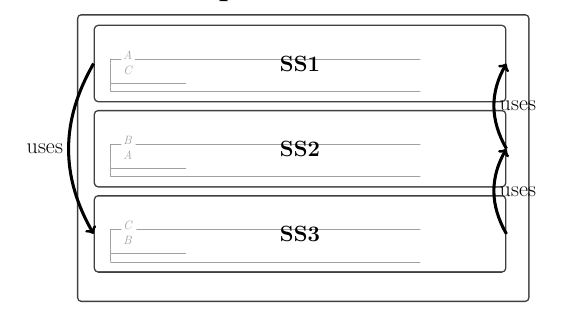
\includegraphics[scale=0.33]{Figures/zdra/zdraloop.png}
\vspace{-0.18in}
\caption{The pdflatex output of figure \ref{fig:aloop}.  \label{fig:zdraerror1}}
\vspace{-0.2in}
\end{minipage}
\end{figure}

Figure \ref{fig:zdraerror1} shows the relationship SS1 \textit{uses} SS3, SS2
\textit{uses} SS1 and SS3 \textit{uses} SS2. The ZDRa would not allow this as
the reasoning would be in a loop and would not be correct. When running the
\gls{zdra} check on this specification the message which would appear is shown
in figure \ref{fig:zdraerrormess}

\begin{figure}[H]
\centering
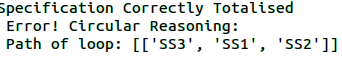
\includegraphics[scale=0.4]{Figures/zdra/loopmessage.png}
\caption{An example of an error message when a specification is not \gls{zdra} correct. \label{fig:zdraerrormess}}
\end{figure}

If the specification is \gls{zdra} correct then the program also creates visual
dependency and GoTo graphs automatically (see section
\ref{subsec:zdra_prodcuts}). If not then the graphs are not created.

A full specification which passes \gls{zcga} is shown in appendix
\ref{app:failzdra}. There is one loop in the reasoning of this specification and
the user is able to see it when they annotated the specification in \gls{zdra}
and have compiled the document using \texttt{pdflatex}. A snippet of this is
shown in figure \ref{fig:zdraloopsnippet} and the full version is shown in
appendix \ref{app:failzdraout}.

\begin{figure}[H]
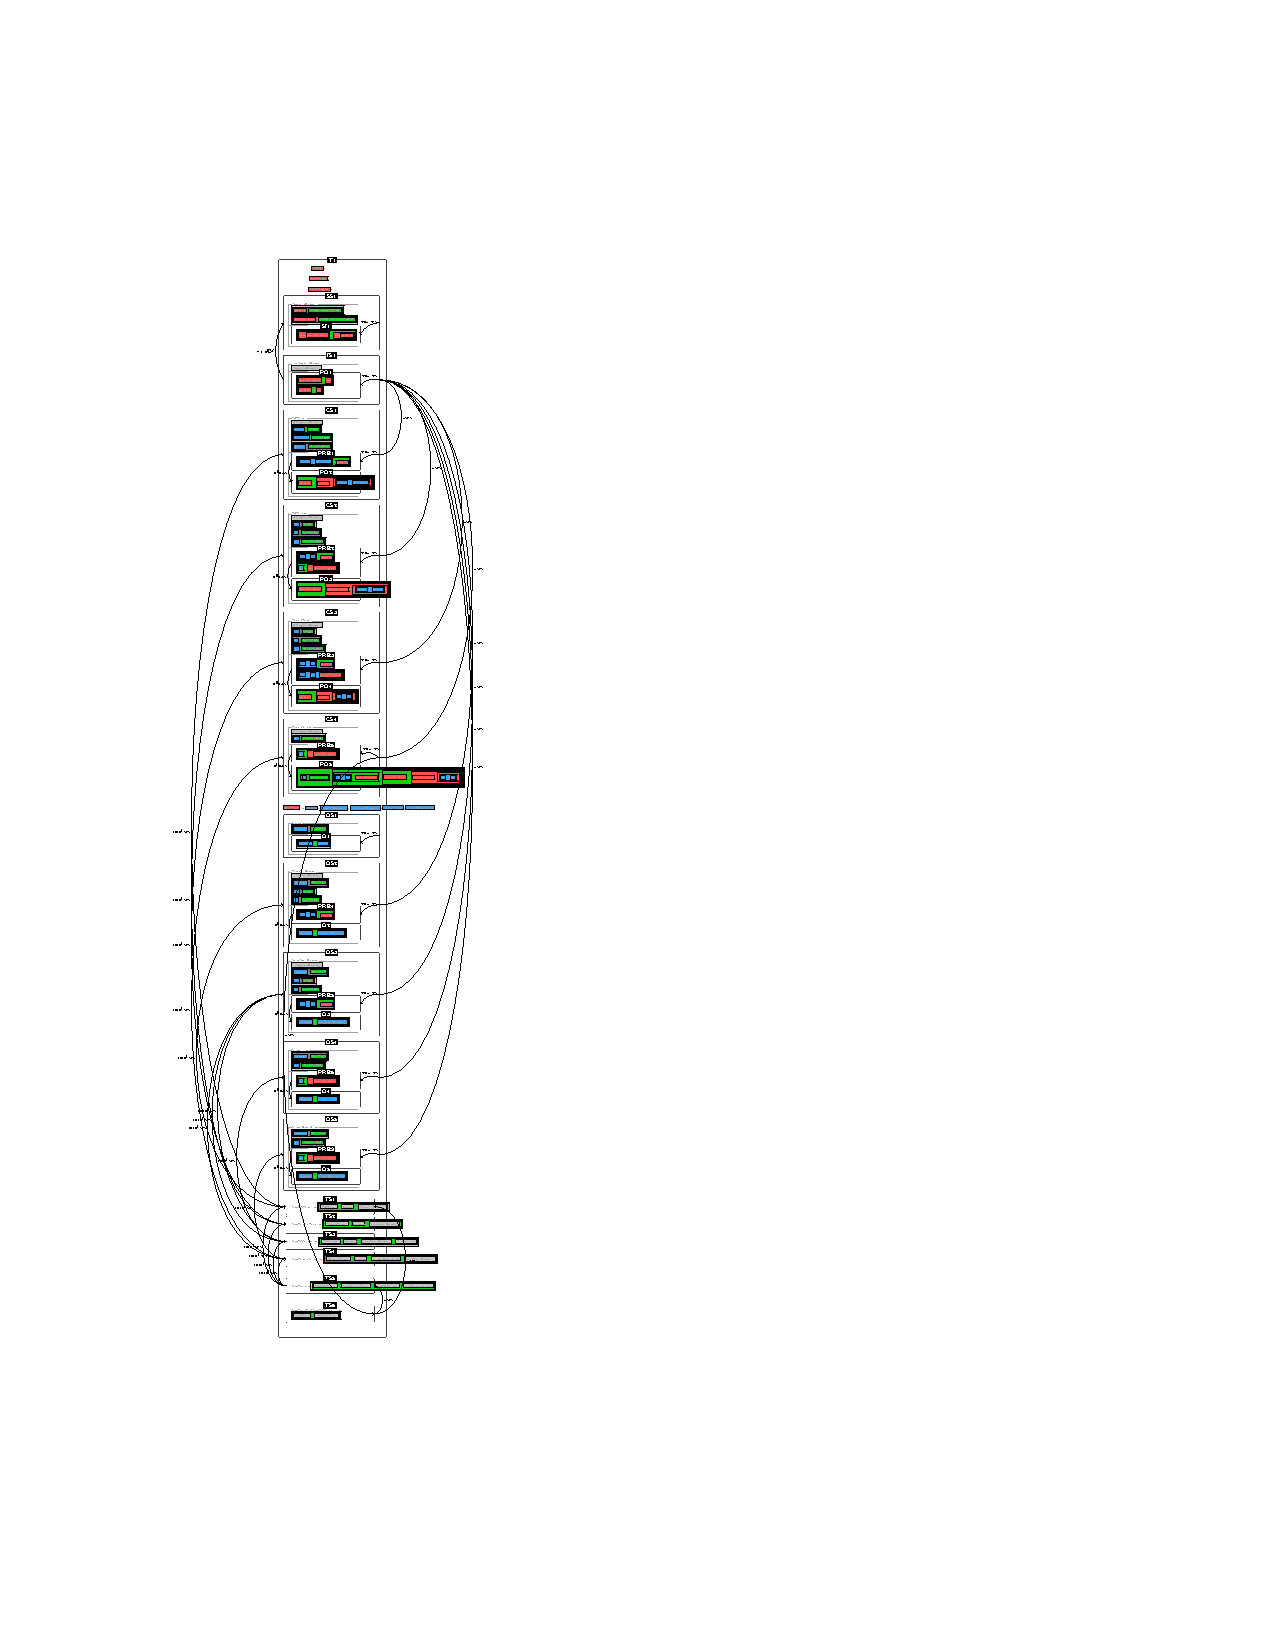
\includegraphics[clip, trim=0cm 10cm 6cm 11cm, scale=1.3]{examples/nonworkzdra/1n2.pdf}
\caption{A snippet from appendix \ref{app:failzdra} showing a loop in reasoning. \label{fig:zdraloopsnippet}}
\end{figure}

When the specification is checked with \gls{zcga} then the output message says
the specification is grammatically correct. However when the specification is
checked with \gls{zdra}, the message says that circular reasoning has been found
and shows the path of the loop, which in this case is \verb|CS4, TS4, TS5, TS6|.
The error message which appears specifically for this example in shown in figure
\ref{app:failzdraoutmessgae} in appendix \ref{app:failzdraoutmes}.

\subsection{Products}
\label{subsec:zdra_prodcuts}

When the specification has been ZDRa checked the program will then output two
new files. 

\begin{enumerate}

\item ZDRa specification Dependency Graph

\item ZDRa specification GoTo Graph
\end{enumerate}

The \gls{zdra} specification Dependency graph uses the labels and annotations
from the \gls{zdra} to show the dependencies between each of the instances. The
ZDRa GoTo graph illustrates which instances are dependent or are needed for
another instance to exist. Both graphs are built using the directed graph built
in the \gls{zdra} check (see section \ref{subsec:loops}). Further information on
how these products are formed can be found in the next chapter.

\subsubsection{Dependency Graph}

\begin{figure}[H]
\centering
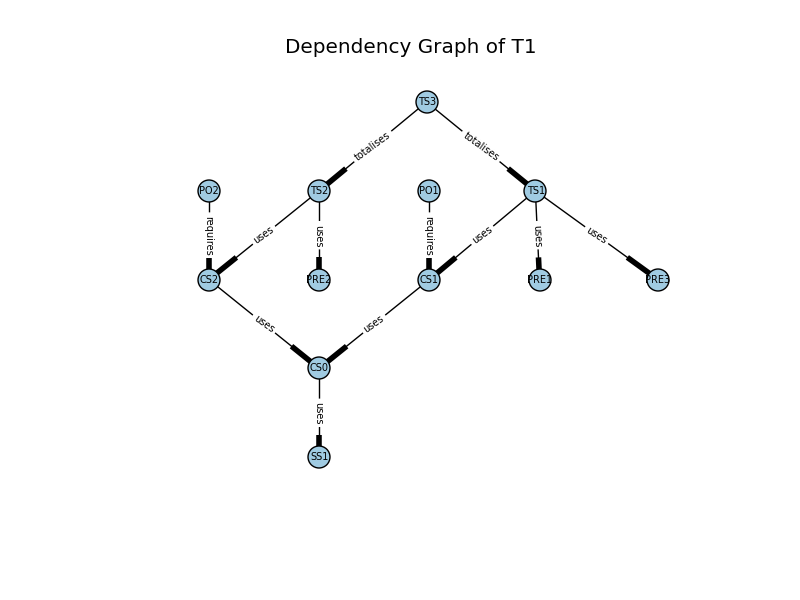
\includegraphics[scale=0.6]{Figures/zdra/depgraph.png}
\caption{An example of a dependency graph. \label{fig:depgraph}}
\end{figure}

An example of a \emph{dependency graph} can be seen in figure
\ref{fig:depgraph}. This image represents the compiled \gls{zdra} annotated
document but it graph form. All the boxes that show up in the compiled document
are represented by nodes in the graph. The arrows from the instances are
represented by the edges in the graph, all the arrows in the document and edges
in the graph should be pointing in the same direction.


\subsubsection{GoTo Graph}

\begin{figure}[H]
\centering
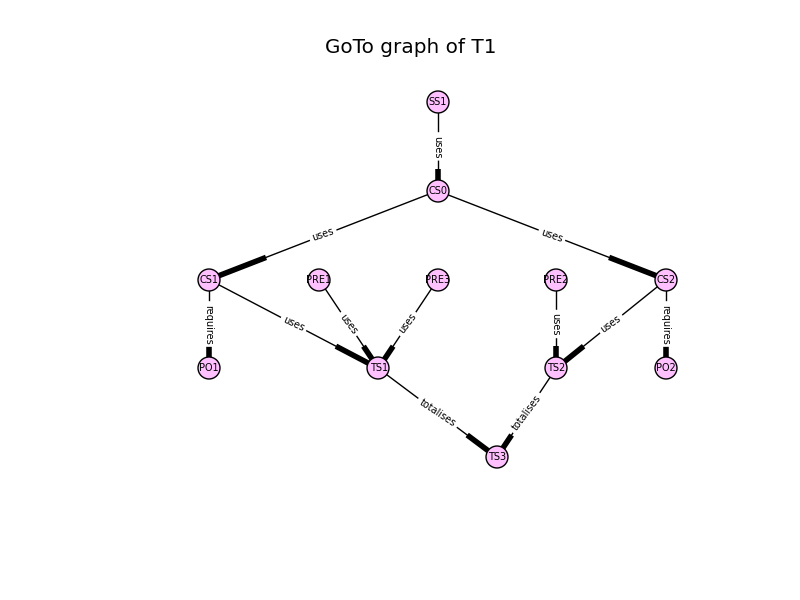
\includegraphics[scale=0.6]{Figures/zdra/gotograph.png}
\caption{An example of a goto graph \gls{zdra} correct. \label{fig:gotograph}}
\end{figure}

An example of a \emph{goto graph} is shown in figure \ref{fig:gotograph}, it is
very similar to the \emph{dependency graph}. The \emph{goto graph} also uses the
boxes created by the \gls{zdra} annotations \verb|draschema| and \verb|draline|.
However the only slight difference is the directions the edges are pointing to
in some of the relations. For example if we had the relation
\verb|\initialOf{IS1}{SS1}|, in the compiled document and in the
\emph{dependency graph} the arrow will be going from \verb|IS1| to \verb|SS1|
this is because it is indeed true that the initial schema \verb|IS1| is the
\textbf{initial of} the state schema \verb|SS1|. On the other hand, in the
\emph{goto graph} the edge is pointing the other way from the stateschema
\verb|SS1| to the initialschema \verb|IS1|. This is because the initialschema
\verb|IS1| needs \verb|SS1| to exist, that is if \verb|SS1| didn't exist then
\verb|IS1| couldn't initialise it. Therfore the instance \verb|IS1| is dependent
on \verb|SS1|.

The other \gls{zdra} relations which also reverse the direction of the arrow in
the \emph{goto graph} are \emph{uses},\emph{requires} and \emph{totalises}.

\section{A formal view on the \gls{zdra}.}

We denote the star character `*' to denote one or many. We remind the reader
that `$\mathbf{\Gamma}$' denotes the schematext of a specification,
$\mathcal{Z}, \mathcal{E}, \mathcal{T}$ and $\mathbb{S}$ are correctly typed
\emph{declatation}, \emph{expression}, \emph{term} and \emph{set} respectively
(from table \ref{tab:zcga1} in chapter \ref{ch:zcga}).

\begin{defin}
Let $\mathcal{E}$ be a correctly typed expression. \\ Let $\mathcal{D}$ be a
correctly typed definition. \\
Where $((\mathcal{Z}@\mathcal{E})$*$|\mathcal{T}$*$|\mathbb{S}$*$) \in
\mathcal{E}$ and $(\mathcal{T}$*$|\mathbb{S}$*$) \in \mathcal{D}$\\
Let $\mathcal{ED}$ be the set containing $\mathcal{E}$'s and $\mathcal{D}$'s.
\end{defin}

For example an expression can be the following: \verb|t = t| where $t$ is a
term. Therefore this expression contains two terms. Another example of an
expression could be: $\forall t: S \bullet t = 0$. This expression contains a
declaration within an expression ($(\mathcal{Z}@\mathcal{E})$, which is $t:S$.


\begin{table}[H]
\begin{footnotesize}
\begin{tabular}{| l | l | l |}
\hline
\textbf{Instance} & \textbf{Allowed weak types} & \textbf{Annotations} \\
\hline
\hline
precondition & $\mathcal{ED} \in \mathbf{\Gamma}$ &
\cgatext{\expression{\mathcal{E}}\definition{\mathcal{D}}} \\

postcondition & $\mathcal{ED} \in \mathbf{\Gamma}$ &
\cgatext{\expression{\mathcal{E}}\definition{\mathcal{D}}} \\

output & $\mathcal{ED} \in \mathbf{\Gamma}$ &
\cgatext{\expression{\mathcal{E}}\definition{\mathcal{D}}} \\

stateInvariants & $\mathcal{ED} \in \mathbf{\Gamma}$ &
\cgatext{\expression{\mathcal{E}}\definition{\mathcal{D}}} \\

stateSchema & $(\mathcal{Z} \& \mathcal{ED}) | \mathcal{Z} \in \mathbf{\Gamma}$
& $(\cgatext{\declaration{\mathcal{Z}$*$} \&
\expression{\mathcal{E}}\definition{\mathcal{D}}}) |
\cgatext{\declaration{\mathcal{Z}$*$}}$ \\

theory & $(\mathcal{Z} \& \mathcal{ED}) | \mathcal{Z} \in \mathbf{\Gamma}$ &
$(\cgatext{\declaration{\mathcal{Z}$*$} \&
\expression{\mathcal{E}}\definition{\mathcal{D}}}) |
\cgatext{\declaration{\mathcal{Z}$*$}}$\\

changeSchema & $(\mathcal{Z} \& \mathcal{ED}) | \mathcal{ED} \in
\mathbf{\Gamma}$ & $(\cgatext{\declaration{\mathcal{Z}$*$} \&
\expression{\mathcal{E}}\definition{\mathcal{D}}}) |
\cgatext{\expression{\mathcal{E}}\definition{\mathcal{D}}}$ \\

totaliseSchema & $(\mathcal{Z} \& \mathcal{ED}) | \mathcal{ED} \in
\mathbf{\Gamma}$ & $(\cgatext{\declaration{\mathcal{Z}$*$} \&
\expression{\mathcal{E}}\definition{\mathcal{D}}}) |
\cgatext{\expression{\mathcal{E}}\definition{\mathcal{D}}}$ \\

axiom & $\mathcal{Z} \& \mathcal{ED} \in \mathbf{\Gamma} $ &
$\cgatext{\declaration{\mathcal{Z}$*$} \&
\expression{\mathcal{E}}\definition{\mathcal{D}}}$ \\

outputSchema & $\mathcal{Z} \& \mathcal{ED} \in \mathbf{\Gamma} $ &
$\cgatext{\declaration{\mathcal{Z}$*$} \&
\expression{\mathcal{E}}\definition{\mathcal{D}}}$ \\

initSchema & $\mathcal{Z} \& \mathcal{ED} \in \mathbf{\Gamma} $ &
$\cgatext{\declaration{\mathcal{Z}$*$} \&
\expression{\mathcal{E}}\definition{\mathcal{D}}}$ \\

\hline
\end{tabular}

\end{footnotesize}
\caption{ZCGa annotations allowed in ZDRa instances \label{tab:zcgainzdra}}
\end{table}

Table \ref{tab:zcgainzdra} shows which \gls{zcga} are allowed to be in certain
\gls{zdra} instances. Where `\&' means these weak type categories must be
included in the instance. For example a \emph{stateSchema} can be made up of one
or more $\mathcal{Z}$ \textbf{AND} one or more $\mathcal{ED}$ \textbf{OR} one or
more $\mathcal{Z}$ on their own. Therefore a \emph{stateSchema} can not be made
up of $\mathcal{ED}$ on it's own.

\paragraph{precondition, postcondition, output, stateInvariants.}
These instances can only contain a correctly typed expression or definition
within the schematext. There may be one or more expressions or definitions.

\paragraph{stateSchema, theory.}
These instances can only contain one or more correctly typed declaration
\emph{and} one or more correctly typed expression and definition or one or more
correctly typed declarations.

\paragraph{changeSchema, totalise.}
These instances can only contain one or more correctly typed declaration
\emph{and} one or more correctly typed expression and definition or one or more
correctly typed expressions or definitions.

\paragraph{axiom, outputSchema, initSchema}
These instances can only contain one or more correctly typed declarations
\emph{and} one or more correctly typed expression and definitions.

\subsection{Allowances when combining the ZCGa and ZDRa}

Since we have formally outlined the \gls{zdra} in table \ref{tab:zcgainzdra} we
can now show some rules which occur when we combing the \gls{zcga} and
\gls{zdra} together.

\begin{thm}
Using table \ref{tab:zcgainzdra}, the initialOf relation only permits the
annotations: \\
 $\mathcal{Z} \& \mathcal{ED}, initialOf, (\mathcal{Z} \& \mathcal{ED}) |
 \mathcal{Z}$.
\end{thm}

\begin{proof}
From table \ref{tab:relationsallowed} (section \ref{subsec:zdrarelations}) we
can see the only legal relation for initialOf is `initSchema $\longrightarrow$
stateSchema'. An initSchema can only have the annotation $\mathcal{Z} \&
\mathcal{ED}$ and a stateSchema can only have the annotations $(\mathcal{Z} \&
\mathcal{ED}) | \mathcal{Z}$ (from table \ref{tab:zcgainzdra}). Since
$\longrightarrow$ represents the relation \emph{initialOf} then we get
$\mathcal{Z} \& \mathcal{ED}, initialOf, ((\mathcal{Z} \& \mathcal{ED}) |
\mathcal{Z})$.
\end{proof}

\begin{thm}
Using table \ref{tab:zcgainzdra}, the allows relation only permits the
annotations: \\
$\mathcal{ED}, allows, \mathcal{ED}$.
\end{thm}

\begin{proof}
The allows relation only permits `precondition $\longrightarrow$ postcondition'
(table \ref{tab:relationsallowed}). Both a precondition and postcondition have
the \gls{zcga} annotations $\mathcal{ED}$. Since $\longrightarrow$ represents
the relation. Then the result is $\mathcal{ED}, allows, \mathcal{ED}$.
\end{proof}

\begin{thm}
Using table \ref{tab:zcgainzdra}, the requires relation only permits the
annotations:
\begin{itemize}
\item $\mathcal{Z} \& \mathcal{ED}, requires, \mathcal{ED}$
\item $(\mathcal{Z} \& \mathcal{ED}) | \mathcal{ED}, requires, \mathcal{ED}$
\end{itemize}
\end{thm}

\begin{proof}
Using table (table \ref{tab:relationsallowed}) of permitted relations the
requires relation has the following syntax:
\begin{enumerate}
\item `outputSchema $\longrightarrow$ precondition'
\item `outputSchema $\longrightarrow$ output', 
\item `changeSchema $\longrightarrow$ precondition', 
\item `changeSchema $\longrightarrow$ postcondition', 
\end{enumerate} 
\begin{itemize}

\item Using the allowed \gls{zcga} annotations in table \ref{tab:zcgainzdra} we
can see that an outputSchema contains only $\mathcal{Z} \& \mathcal{ED}$ and a
precondition and output both only contain $\mathcal{ED}$ thus 1 and 2 become
$\mathcal{Z} \& \mathcal{ED} \longrightarrow \mathcal{ED}$. Since
$\longrightarrow$ represents the relation then we end up with $\mathcal{Z} \&
\mathcal{ED}, requires, \mathcal{ED}$.

\item The allowed \gls{zcga} annotations for changeSchema are $(\mathcal{Z} \&
\mathcal{ED}) | \mathcal{ED}$ and the allowed \gls{zcga} annotations for both
precondition and postcondition are $\mathcal{ED}$ therefore we end up with
($(\mathcal{Z} \& \mathcal{ED}) | \mathcal{ED} \longrightarrow \mathcal{ED}$.
Again the $\longrightarrow$ represents the relation so the $\longrightarrow$
becomes `requires' and we are left with $(\mathcal{Z} \& \mathcal{ED}) |
\mathcal{ED}, requires, \mathcal{ED}$.
\end{itemize}
\end{proof}

\begin{thm}
Using table \ref{tab:zcgainzdra}, the totalises relation only permits the
annotations:
\begin{itemize}
\item $(\mathcal{Z} \& \mathcal{ED}) | \mathcal{ED}), totalises, (\mathcal{Z} \&
\mathcal{ED}) | \mathcal{ED}$
\item $(\mathcal{Z} \& \mathcal{ED}) | \mathcal{ED}), totalises, \mathcal{Z} \&
\mathcal{ED}$
\end{itemize}
\end{thm}

\begin{proof}
Using table (table \ref{tab:relationsallowed}) of permitted relations the
totalises relation has the following syntax:
\begin{enumerate}
\item `totaliseSchema $\longrightarrow$ changeSchema'
\item `totaliseSchema $\longrightarrow$ outputSchema'
\item `totaliseSchema $\longrightarrow$ totaliseSchema'
\end{enumerate} 

\begin{itemize}
\item Table \ref{tab:relationsallowed} shows the \gls{zcga} syntax for
totaliseSchema and changeSchema is $(\mathcal{Z} \& \mathcal{ED}) |
\mathcal{ED})$. Thus the permitted relations would be $(\mathcal{Z} \&
\mathcal{ED}) | \mathcal{ED}) \longrightarrow (\mathcal{Z} \& \mathcal{ED}) |
\mathcal{ED})$ for points 1 and 3. Since $\longrightarrow$ represents the
relation `totalises' in this case we would have $(\mathcal{Z} \& \mathcal{ED}) |
\mathcal{ED}), totalises, (\mathcal{Z} \& \mathcal{ED}) | \mathcal{ED})$. Hence
the first part of the theorem is proven.

\item Output schema has the \gls{zcga} sytntax $(\mathcal{Z} \& \mathcal{ED})$
according to table \ref{tab:zcgainzdra}. If totaliseSchema has the \gls{zcga}
syntax $(\mathcal{Z} \& \mathcal{ED}) | \mathcal{ED})$ then using point 2 the
permitted relation would be $(\mathcal{Z} \& \mathcal{ED}) | \mathcal{ED})
\longrightarrow \mathcal{Z} \& \mathcal{ED}$. Again since $\longrightarrow$
represent totalise in this case we conclude with $(\mathcal{Z} \& \mathcal{ED})
| \mathcal{ED}), totalises, \mathcal{Z} \& \mathcal{ED}$.
\end{itemize}
\end{proof}

\begin{thm}
Using table \ref{tab:zcgainzdra}, the uses relation only permits the
annotations:
\begin{itemize}
\item $\mathcal{Z} \& \mathcal{ED}, uses, (\mathcal{Z} \& \mathcal{ED}) |
\mathcal{Z}$
\item $(\mathcal{Z} \& \mathcal{ED}) | \mathcal{ED}, uses, (\mathcal{Z} \&
\mathcal{ED}) | \mathcal{Z}$
\item $(\mathcal{Z} \& \mathcal{ED}) | \mathcal{Z}, uses, (\mathcal{Z} \&
\mathcal{ED}) | \mathcal{Z}$
\item $(\mathcal{Z} \& \mathcal{ED}) | \mathcal{Z}, uses, \mathcal{Z} \&
\mathcal{ED}$
\item $\mathcal{Z} \& \mathcal{ED}, uses, \mathcal{Z} \& \mathcal{ED}$
\item $(\mathcal{Z} \& \mathcal{ED}) | \mathcal{ED}, uses, \mathcal{Z} \&
\mathcal{ED}$
\end{itemize}
\end{thm}

\begin{proof}
Using table (table \ref{tab:relationsallowed}) of permitted relations the uses
relation has the following syntax:
\begin{enumerate}
\item `outputSchema $\longrightarrow$ stateSchema'
\item `changeSchema $\longrightarrow$ stateSchema'
\item `stateSchema $\longrightarrow$ stateSchema'
\item `stateSchema $\longrightarrow$ axiom'
\item `outputSchema $\longrightarrow$ axiom'
\item `changeSchema $\longrightarrow$ axiom'
\end{enumerate} 

\begin{itemize}
\item According to table \ref{tab:zcgainzdra} the \gls{zcga} syntax for
outputSchema is $\mathcal{Z}\&\mathcal{ED}$ and the syntax for stateSchema is
$(\mathcal{Z} \& \mathcal{ED}) | \mathcal{Z}$. Therefore using point 1 we get
`$\mathcal{Z}\&\mathcal{ED} \longrightarrow (\mathcal{Z} \& \mathcal{ED}) |
\mathcal{Z}$'. Since $\longrightarrow$ represents the relation uses in this case
we get $\mathcal{Z} \& \mathcal{ED}, uses, (\mathcal{Z} \& \mathcal{ED}) |
\mathcal{Z}$.

\item The syntax for changeSchema is $(\mathcal{Z} \& \mathcal{ED}) |
\mathcal{ED}$ and the syntax for stateSchema is $(\mathcal{Z} \& \mathcal{ED}) |
\mathcal{Z}$ according from table \ref{tab:zcgainzdra}. Substituting the
\gls{zcga} for instance names in point 2 we get $(\mathcal{Z} \& \mathcal{ED}) |
\mathcal{ED} \longrightarrow (\mathcal{Z} \& \mathcal{ED}) | \mathcal{Z}$. By
substituting the relation uses for $\longrightarrow$ we end up with
$(\mathcal{Z} \& \mathcal{ED}) | \mathcal{ED}, uses, (\mathcal{Z} \&
\mathcal{ED}) | \mathcal{Z}$.

\item Using table \ref{tab:zcgainzdra} the \gls{zcga} syntax for stateSchema is
$(\mathcal{Z} \& \mathcal{ED}) | \mathcal{Z}$. Using point 3, we substitute the
\gls{zcga} syntax for the instance name and we get $(\mathcal{Z} \&
\mathcal{ED}) | \mathcal{Z} \longrightarrow (\mathcal{Z} \& \mathcal{ED}) |
\mathcal{Z}$. Since $\longrightarrow$ represents uses then we get $(\mathcal{Z}
\& \mathcal{ED}) | \mathcal{Z}, uses, (\mathcal{Z} \& \mathcal{ED}) |
\mathcal{Z}$.

\item The \gls{zcga} syntax for stateSchema is $(\mathcal{Z} \& \mathcal{ED}) |
\mathcal{Z}$ and the \gls{zcga} syntax for axiom is  $\mathcal{Z} \&
\mathcal{ED}$. By subsituting these \gls{zcga} syntax's in point 4 we get
$(\mathcal{Z} \& \mathcal{ED}) | \mathcal{Z} \longrightarrow \mathcal{Z} \&
\mathcal{ED}$. Since $\longrightarrow$ in this case is the relationship uses, we
can change $\longrightarrow$ to `uses' and get $(\mathcal{Z} \& \mathcal{ED}) |
\mathcal{Z}, uses, \mathcal{Z} \& \mathcal{ED}$.

\item According to table \ref{tab:zcgainzdra} the \gls{zcga} syntax for
outputSchema and axiom are both $\mathcal{Z} \& \mathcal{ED}$. Therefore if we
put in the \gls{zcga} syntax instead of the instance names in point 5 we get
$\mathcal{Z} \& \mathcal{ED} \longrightarrow \mathcal{Z} \& \mathcal{ED}$. From
table \ref{tab:relationsallowed} we can deduce that $\longrightarrow$ mean
`uses' so we finish with $\mathcal{Z} \& \mathcal{ED}, uses, \mathcal{Z} \&
\mathcal{ED}$.

\item Finally, the \gls{zcga} syntax for changeSchema is $(\mathcal{Z} \&
\mathcal{ED}) | \mathcal{ED}$ and the \gls{zcga} syntax for axiom is
$\mathcal{Z} \& \mathcal{ED}$ according to table \ref{tab:zcgainzdra}. If we
substitute the allowed \gls{zcga} syntax in point 6 we get $(\mathcal{Z} \&
\mathcal{ED}) | \mathcal{ED} \longrightarrow \mathcal{Z} \& \mathcal{ED}$. Since
$\longrightarrow$ is the relation `uses' in this case we end up with
$(\mathcal{Z} \& \mathcal{ED}) | \mathcal{ED}, uses, \mathcal{Z} \&
\mathcal{ED}$.
\end{itemize}
\end{proof}

\section{Conclusion}
In this chapter the \gls{zdra} step of the \gls{zmath} has been described. A
\LaTeX{} style package has been created to allow a user to annotate a Z
specification and see the structure of the system. A \gls{zdra} program has been
created to check for rhetorical correctness and make sure there are no loops in
the reasoning of the specification. Warning messages appear if the specification
is still lacking some totalising schemas for some preconditions. We have also
formally outlined the \gls{zdra} and shown some rules which occur when combining
the \gls{zcga} and \gls{zdra} together. If the specification is correct at the
\gls{zdra} stage then the user may then go on to create general and theorem
prover specific skeletons which are described in the next chapter.